\subsection{Praktische Anwendung der FM-Synthese}
\subsubsection{Nachbildung eines Instruments}
Da es bei der FM Synthese schwer möglich ist im Vorfeld zu wissen was für ein Signal herauskommt. Ist es schwer mit dieser Technik ein echt wirkendes Instrument nachzubilden.
Trotzdem gibt es einige Methoden den generierten Klang natürlicher wirken zu lassen. Diese werden im weiteren Verlauf diese Kapitels vorgestellt und anschließend versucht den Klang eines Instruments nachzubilden.

Hüllkurven
Da bei vielen Instrumenten die Lautstärke während der Laufzeit eines Tones variiert, und ein abruptes Ein oder Ausschalten des Tones nicht besonders real klingt, ist die Nutzung einer Hüllkurve oder ADSR-Hüllkurve ein wichtiger Bestandteil der Nachbildung eines Instrumentes. ADSR steht für die einzelnen Phasen eines Tons: Attack, Decay, Sustain und Release. Diese Phasen sollen hier vereinfacht erklärt werden. Beim Drücken einer Taste wird der Ton angeschlagen und die Lautstärke des Tons steigt schnell bis zu einem maximal Wert an. Diese Phase wird Attack-Phase genannt. Nachdem die maximale Lautstärke erreicht wurde, startet die Decay Phase. In dieser Phase sinkt die Lautstärke schnell auf einen geringeren Wert ab. Danach befindet sich der Ton in der Sustain Phase und die Lautstärke bleibt gleich, solange der Ton gespielt wird. Sobald die Taste losgelassen wird, nimmt die Lautstärke wieder bis zu ihrem minimal Wert ab. In Abbildung \ref{fig:defaultADSR} ist der Verlauf der Lautstärke einer Standard ADSR-Hüllkurve noch einmal grafisch dargestellt.

\begin{figure} [ht]
\centering
  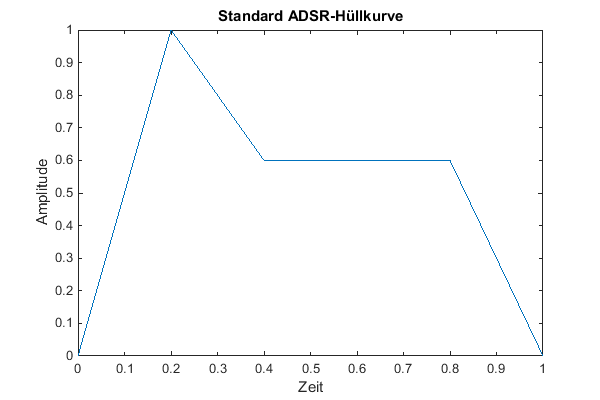
\includegraphics[width=0.95\textwidth]{standardadsr.png}
\caption{Standard ADSR-Hüllkurve}
\label{fig:defaultADSR}
Quelle: Eigene Darstellung mit Matlab
\end{figure}



Da allerdings bei vielen Instrumenten die Lautstärke in den einzelnen Phasen der ADSR-Hüllkurve nicht gleichmäßig steigt oder sinkt, ist es nötig die Kurven zu variieren. Dadurch können Hüllkurven beliebig komplex gestaltet werden. Zum Beispiel steigt bei vielen Instrumenten die Lautstärke in der Attack Phase exponentiell an und fällt in der Decay und Release Phase auch exponentiell ab. Manche Synthesizer bieten zusätzlich auch noch eine Hold Phase vor der Attack Phase, da manche Instrumente einige Zeit benötigen bis sie nach dem Anschlagen des Tones in die Attack Phase eintreten. In Abbildung \ref{fig:blechblasadsr} und \ref{fig:klavieradsr} finden sie weitere für Instrumenten typische Hüllkurven.

\begin{figure} [ht]
\centering
  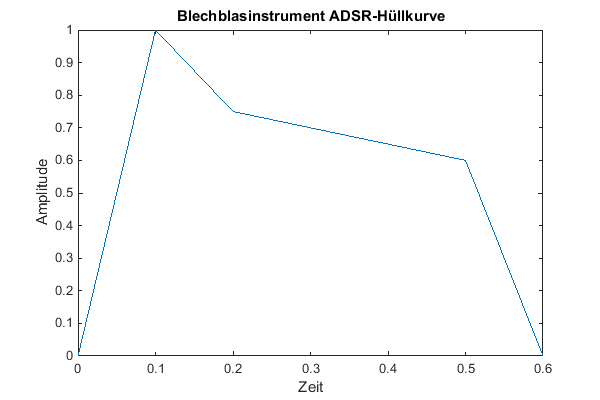
\includegraphics[width=0.95\textwidth]{blechblasadsr.png}
\caption{Typische ADSR-Hüllkurve eines Blechblasinstrumentes}
\label{fig:blechblasadsr}
Quelle: Eigene Darstellung mit Matlab
\end{figure}


\begin{figure} [ht]
\centering
  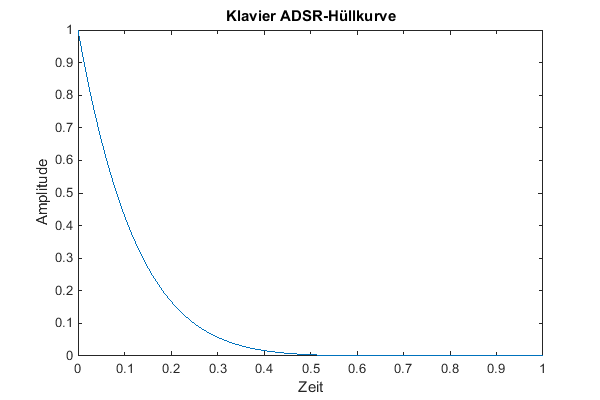
\includegraphics[width=0.95\textwidth]{klavieradsr.png}
\caption{Typische ADSR-Hüllkurve eines Klaviers}
\label{fig:klavieradsr}
Quelle: Eigene Darstellung mit Matlab
\end{figure}


Variabler Modulationsindex
Auch wenn das Hinzufügen einer ADSR-Hüllkurve den Klang des synthetisierten Tones schon stark verbessert, hört sich der erzeugte Ton leider noch nicht wie ein echtes Instrument an. Um den Ton weiter zu verbessern, kann der Modulationsindex über die Zeit oder die Amplitude variiert werden und somit die Anzahl der Seitenfrequenzen verändert werden. Bei Blasinstrumenten wird der Modulationsindex typischerweise über die Amplitude (also mit der ADSR-Hüllkurve) variiert. [Chowning S532]

Wahl der richtigen Modulation
Abgesehen von der einfachen Frequenz Modulation ist es auch möglich mehrere Modulatoren zu verwenden. Diese können in reihe oder parallel geschaltet werden. Außerdem kann auch die sogenannte Feedback Frequenz Modulation genutzt werden, welche das vorran gegangene Signal moduliert. Feedback FM kann vorallem eingesetzt werden um rauschen zu erzeugen. Komplexe FM-Synthese findet Einsatz wenn die normale FM-Synthese nicht mehr aussreicht. Dies kann der Fall sein wenn mehrere stetig fallende Seitenfrequenzen erzeugt werden sollen. Wenn bei einfacher FM-Synthese der Modulationsindex erhöht wird um mehr Seitenfrequenzen zu erzeugen, nimmt die Stärke der Grundfrequenz - definiert durch die Bessel Funktion - immer weiter ab und verteilt sich auf die Seitenfrequenzen  (zu sehen in Fig bla im Kapitel bla). Um dies zu vermeiden können die Modulatoren verschachtelt werden - nachzulesen im Kapitel Komplexe Frequenzmodulation (bla)

Filter
Eine reihe an Filtern kann genutzt werden um das von der FM Synthese erzeugte Signal zu verbessern. Diese Filter können mittels additive oder subtraktive Synthese das Signal manipulieren und so zum Beispiel ungewollte Frequenzen herausfiltern. Typische Filter sind: Hochpassfilter, Tiefpassfilter, Formantenfilter(Rauschen mit der Grundfrequenz und den Harmonischen Vielfachen filtern), 

Einschwingvorgang
Jedes Instrument hat seine eigene charakteristische Einschwingphase, bei vielen Instrumenten ist es eine kurze Hold Phase, die mittels ADSR-Hüllkurve realisiert werden kann.

Noise
Kein Instrument erzeugt einen hundertprozentigen Klang. Bei Luftverwirblungen und Unebenheiten des Instruments wird Rauschen erzeugt. Dieses Rauschen trägt zum typischen Klangbild eines Instruments bei und sollte wenn möglich auch nachgebildet werden. Hierbei kann ein FM Feedback Generator nützlich sein.

Raumhall
Um den Klang des Synthetisierten Tones noch zu realistischer zu machen, kann er mit einem Raumhall veredelt werden.


Beispiel Querflöte
Im Laufe diese Kapitels soll ein Ton einer Querflöte mittels FM-Synthese erzeugt und mit den oben beschriebenen Techniken verfeinert werden. Alle Beispiele sind in Matlab erstellt und können mit den beiliegenden Dateien nachgestellt werden.






Beispiel Klavier

Anhand des Spektrums ist zu erkennen das der Höchste Ausschlag bei 220Hz erfolgt was einem A3 entspricht. Außerdem sind 15 Seitenfrequenzen in einem Abstand von jeweils 220Hz zu erkennen. Aus der Amplituden Plotting lässt sich die ADSR-Hüllkurve ableiten welche sich von 0 bis 0.1 Sekunde in der Attack Phase befindet und ab 0.1 Sekunde bis 1.5 Sekunden in der Decay Phase.



FM Parametrisierung mittels Genetischer Algorithmen
Mittels genetischer Algorithmen ist es möglich Parameter der FM Synthese herauszufinden, die nötig sind um einen Ton zu erzeugen der nach einem Instrument klingt. Diese Algorithmen zerlegen eine Original Ton eines Instrumentes mittels Schneller Fourier Transformation in seine einzelnen Bestandteile und versucht verschiedene Parameter für die Synthese aus, zerlegt das entstandene Signal wieder mittels Schneller Fourier Transformation und vergleicht die Ergebnisse. Mittels dieses Verfahrens können recht zuverlässig Synthetisierte Töne erzeugt werden, die von einem Originalen Instrument kaum zu unterscheiden sind. Da für die Implementierung eines solchen Algorithmus allerdings die Zeit fehlt, wird dieses Thema in dieser Arbeit nicht weiter vertieft. Eine Ausführliche Erklärung der FM Parametrisierung mittels Genetischer Algorithmen kann in Andrew Horners Artikel "Nested Modulator and Feedback FM Matching of Instrument Tones" nachgelesen werden.


Doppel Modulator FM
x(t) = w(t) sin[2*pi*fc*t + Im1*sin(2*pi*fm1*t) + Im2*sin(2*pi*fm2*t)];

Geschachtelte FM Modulation
x(t) = w(t)*sin{2*pi*fc*t + Im1*sin[2*pi*fm1*t + Im2*sin(2*pi*fm2*t)]}

Feedback FM 
xn = wn *sin[(2*pi*f1n/SR)+(B*xn-1/wn-1)]


\subsubsection{Modulationsframework (Theorie -> Praxis)}
\subsubsection{Demo: Parameter und Effekte - Grafiken (evtl. Plotten)}